\section{Software Architecture}

\subsection{Our Aims}

We want to reach these architectural aims:
\begin{enumerate}
	\item hierarchical and distributed system\\
	(e.g. separated Motor-Control)
	\item self-maintaining car \\
	(PID calibration, no hardcoded constants, ...)
	\item simple programming of the master-controller (Linux-PC)
\end{enumerate}

\subsubsection{Hierarchical and distributed system}

The system has to be distributed because of the given hardware structure. The system functionality is distributed over the four Nios2 embedded processors running inside the FPGA boars and the central processor board. All in all we have five operators participating in a star like architecture.\\

The functionality is not only distributed horizontally (over the hardware) but also vertically. This means that there are at least five abstraction layers:
\begin{itemize}
	\item user
	\item central processor board
	\item Nios2 layer
	\item programmable hardware IP-cores in the FPGAs
	\item hardware
\end{itemize}

The program running on the Nios2 processor can only interact with the IP-(Intellectual Property) cores and can exchange some data with the central processor board. The communication between Nios2 processors and the central processor must be limited because of the small data rate of RS232.\\
This limitation leads to a higher responsibility of the lower layers. The Nios2 is the only one who can control speed and sensors which are directly connected to the FPGA. The central processor can at least set the desired speed but has no influence on the controlling itself. Same counts for all layers.\\

To sum up, the distributed system gets the best out of all operators and the hierarchical structure gives us the possibility to limit communication traffic on the network.

\subsubsection{Self-maintaining car}

The car should be able to 'explore' itself. Therefor no constants except for the hardware required are coded. One example is the PID calibration. The user has the possibility to calibrate the PID controller or use the PID values from the last measurement (not implemented yet). This is especially interesting if the car weight has changed (more/less sensors).

\subsubsection{Simple programming}

It would be great if the central processor is simply programmable. For this issue, we use Debian as a well known operation system. You may be able to use more abstract languages for path finding and planing such as Prolog.\\

We also started a 'Wizard' to generate the needed c files for networking. It haven't been completed by now.

\subsection{CMW-Unit SW design} 

Processing Unit: \textsl{Nios II} embedded core.\\	
Main tasks:
\begin{enumerate}
	\item Controlling the motor-speed (PI-Controller)
	\item Communicate with Central-Linux-PC
	\item Polling the sensors
\end{enumerate}

Doing this tasks in a \textbf{hard timed cycle} as required for a real-time system (see \ref{StartMajor}).

\subsubsection{Start sequence}

\begin{figure}[ht]
	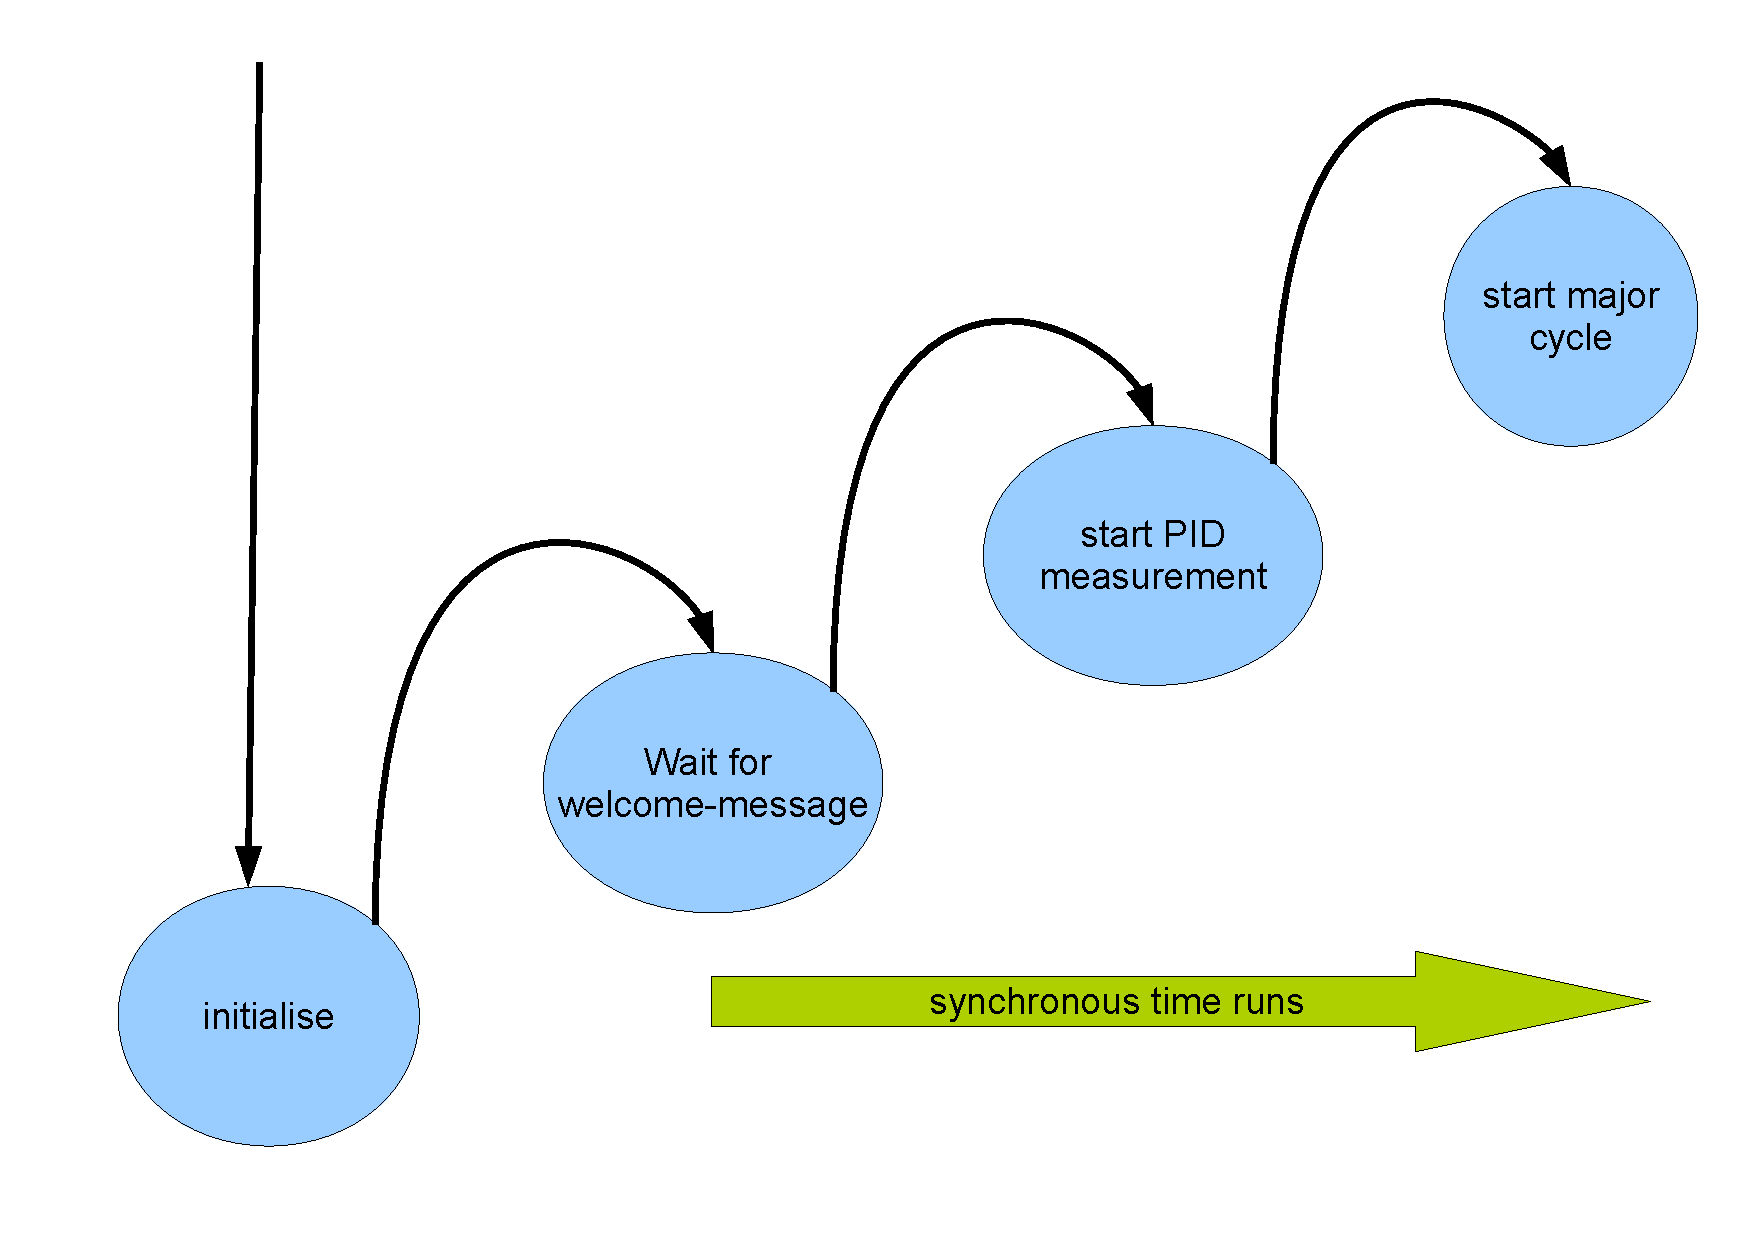
\includegraphics[width=0.5\textwidth]{figures/start.pdf}
	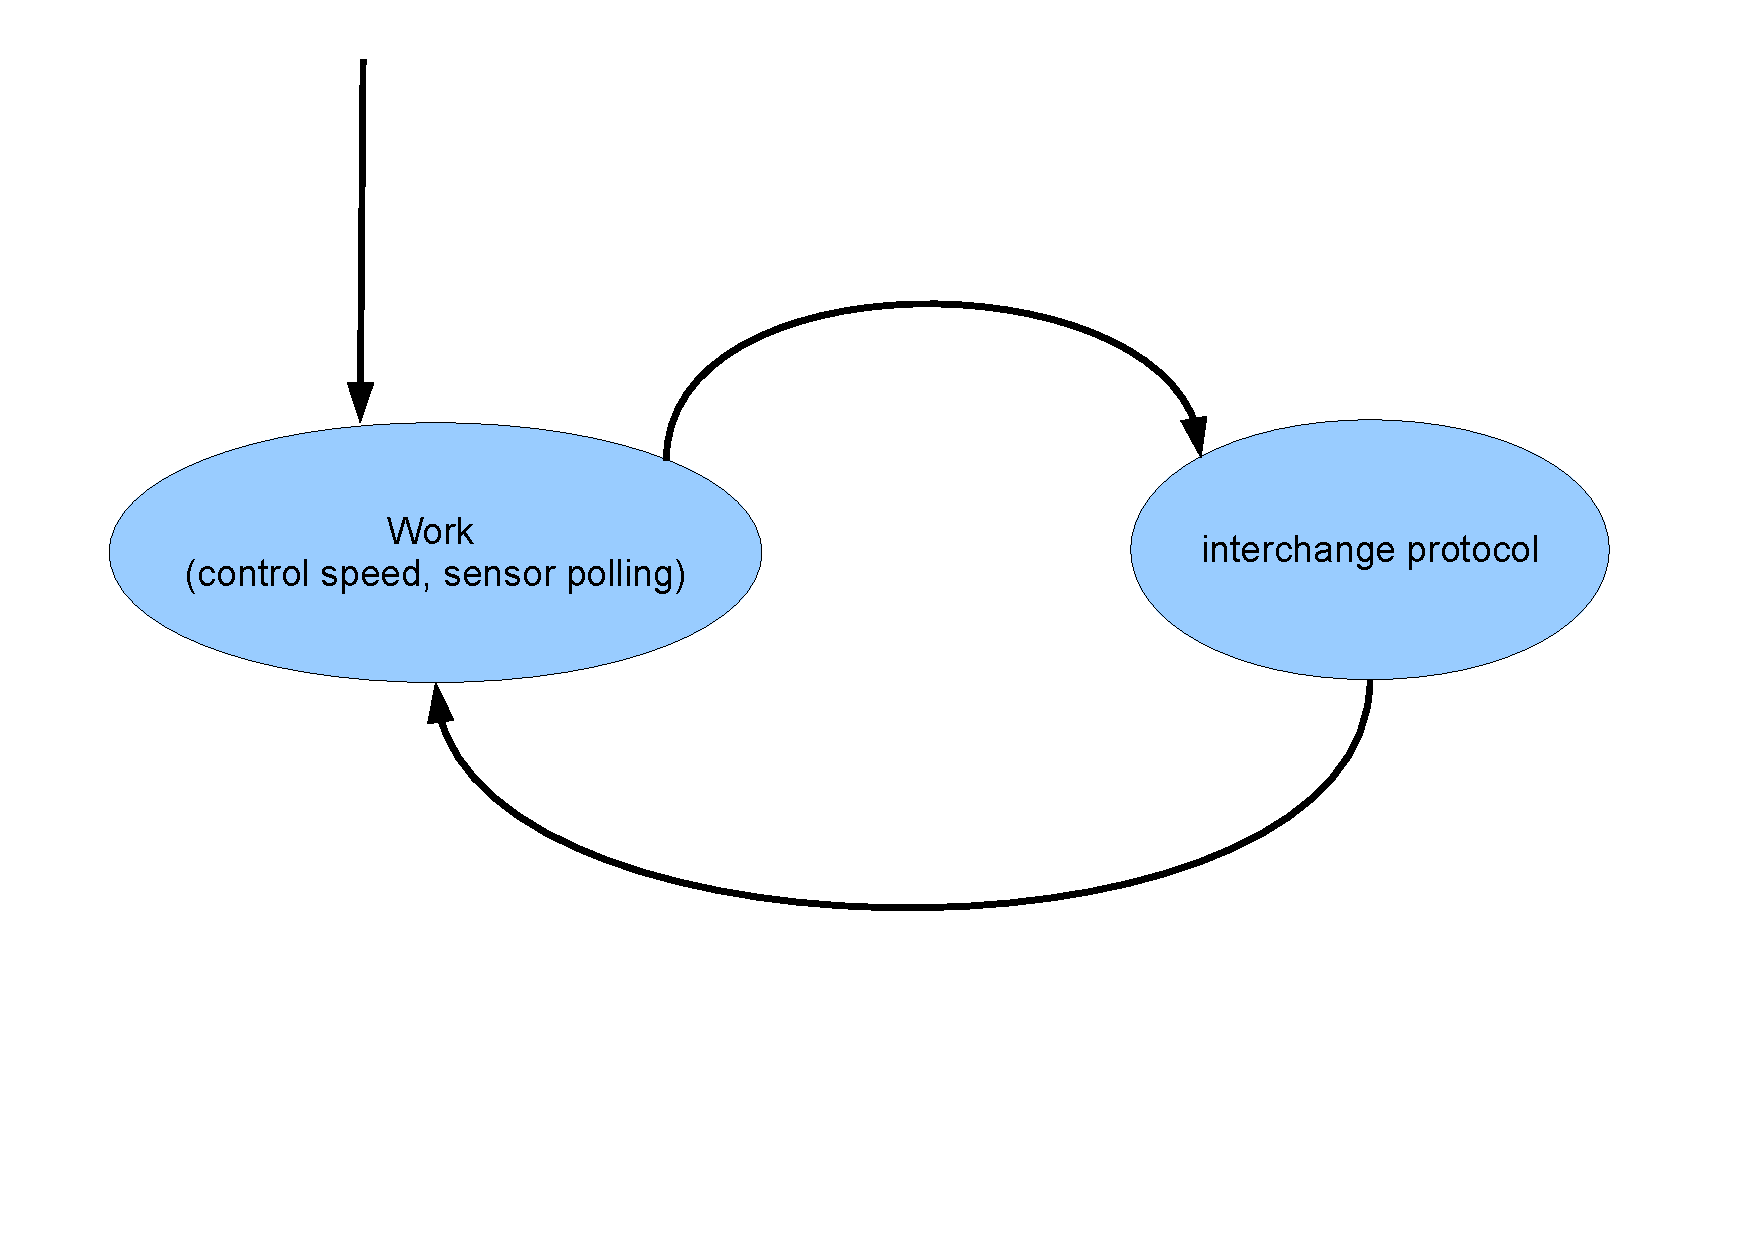
\includegraphics[width=0.5\textwidth]{figures/majorcycle.pdf}
	\caption{Left: Start sequence. Right: Major (or big) cycle.} \label{StartMajor}
\end{figure}

States described in detail:
\begin{itemize}
\item Initialise: Set global fields to zero.
\item Wait for welcome-message:\\
Wait for the first WelcomeMessage. This is necessary to synchronize the Motor-ECUs. After this point every Motor-ECU should be nearly (theoretical clk) synchronous.\\
Note: Due to the nature of TCP over Eth and the Eth2UART there is no guarantee that the ECUs work synchronous but the probability to do so is very high.
\item Start PID measurement:\\
Gets the P-, I- and D-Values for the PID controller by measurement or from the central ECU (Linux-PC) (second option not implemented yet). \\
Note: The motors have a PT1 behavior so there is only a PI controller needed. The D-Value will be ignored (see also \ref{pt1}).

\item Exit on fail:\\
On every fail the speed is set to 0.\\
Important Note: The central ECU is only informed about the failure because it gets no
response from the Motor-ECU. Worst case (if you want to stop also the other motors) is
			\begin{enumerate}
				\item CENTRAL to FAILED MOTOR: regular messages
                \item after 100 ms no response
                \item CENTRAL to all: stop
                \item after TCP / UART delay: motors try to stop
                \item after braking distance the car will be stopped
			\end{enumerate}
The whole process can take about 500 ms!
\end{itemize}

\subsubsection{Major cycle}

Cycle of exact 100 ms (+- a few clock cylces). Every run of this big cycle consists ten smaller cycle runs (see \ref{small}). Task of the big cycle is the network communication which is hard timed to the 100 ms. This means that every 100 ms there should be a new request from the central ECU and the last request is answered. A message round-trip will take aprox. 100 ms + 2TCP/UART delay. Don't forget that TCP/UART is not real-timed!\\

Each of the small cycle runs controls the speed and handles one message (doAction) or waits for a new packet.\\
Note: The big cycle does nothing but merges the small ones!

\subsubsection{Small cycle}

\begin{figure}[ht] 
	\center{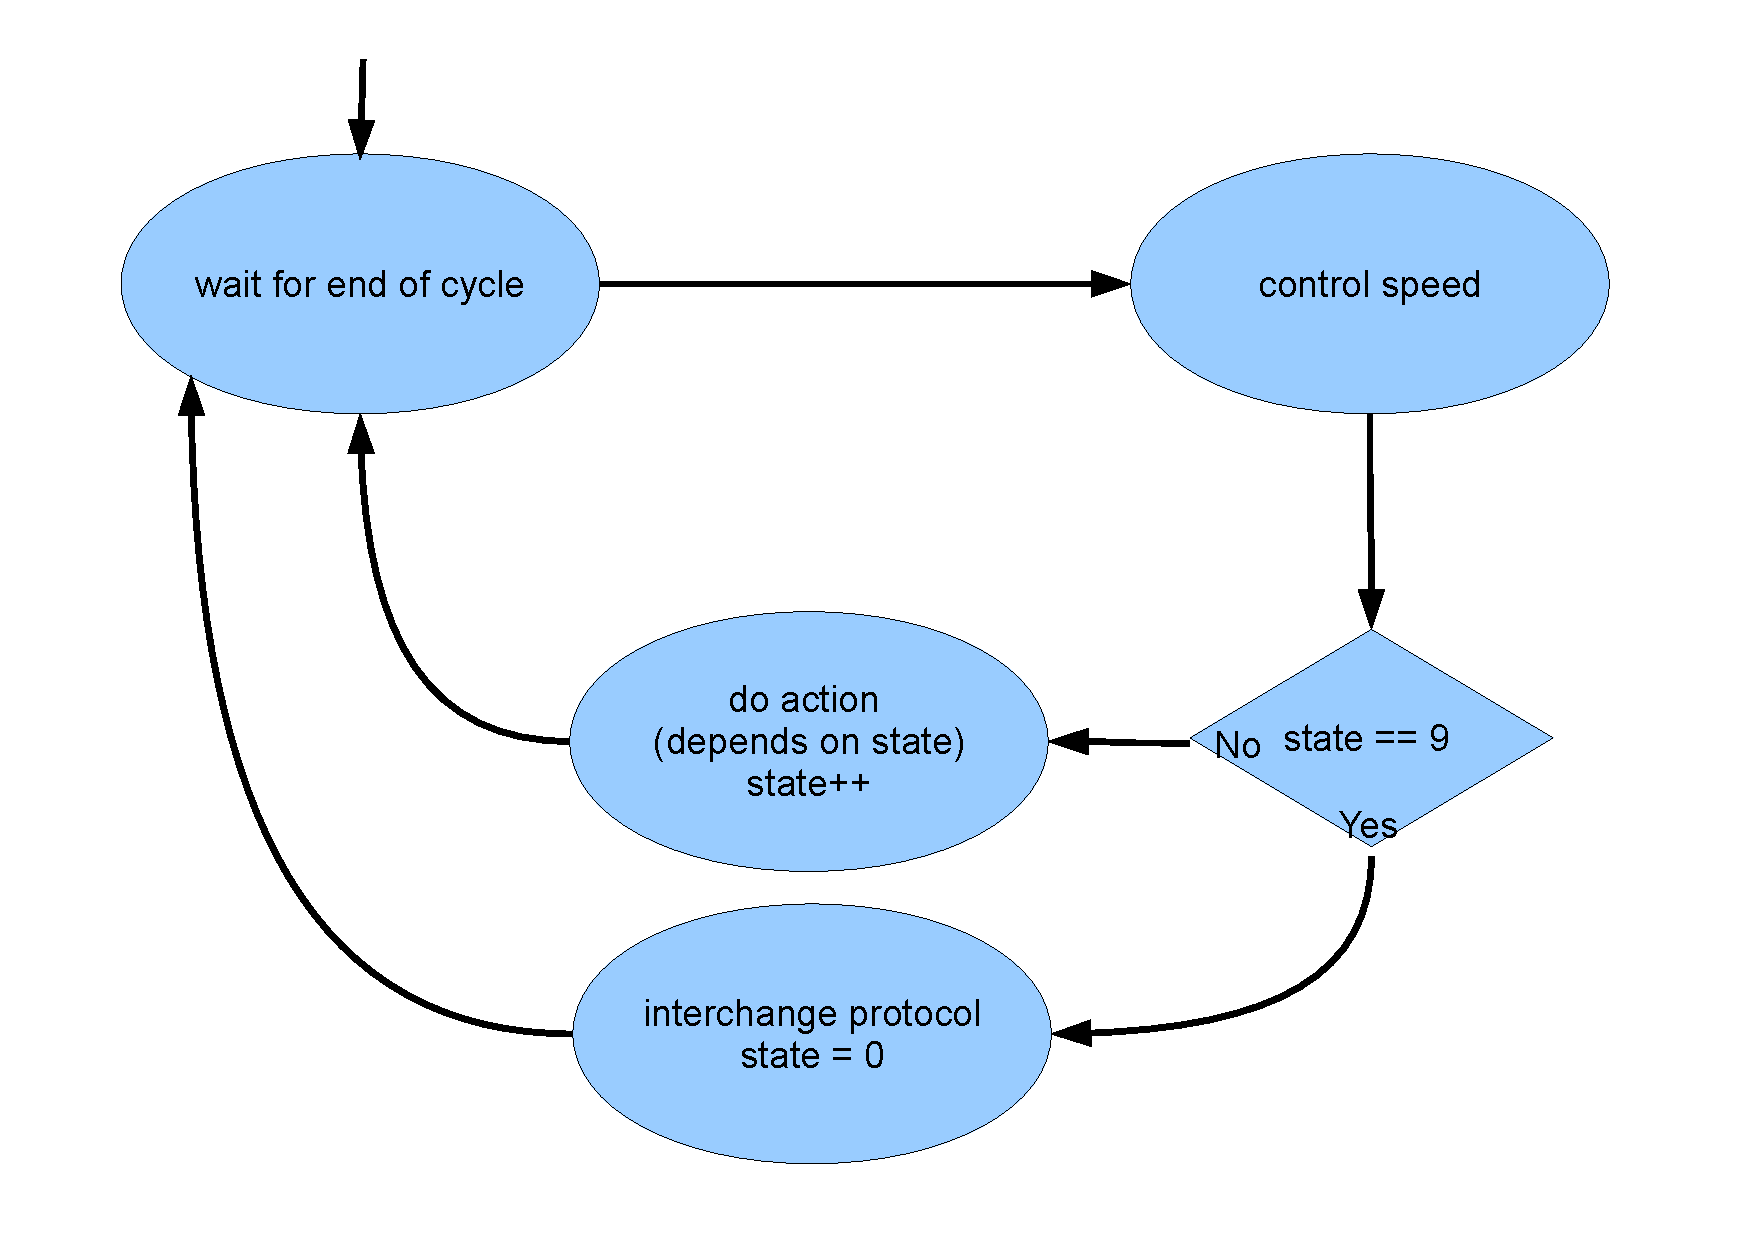
\includegraphics[width=0.5\textwidth]{figures/cycle.pdf}}
	\caption{Small (or minor) cycle.} \label{small}
\end{figure}

States described in detail:
\begin{itemize}
\item wait for end of cycle:\\
The big cycle takes always 100ms, so the ten small cycles take each 10ms. At the begin of a small cycle run a timer is set to this 10ms. WaitForEndOfCycle will block until this timer reached 0. After that the timer is automatically set back to 10ms.\\

Note: The hard timing only works if the rest of the small cycle (including the doAction() method) doesn't take longer than 10 ms. There should be even a security window of 1-2ms!\\
Don't forget that 'control speed' itself takes some of the 10 ms. So said there are only 4-5 ms remaining for your doAction()!

\item control speed:\\
The speed measurement takes place during the whole small cycle run. To get reliable measurement results this state has to be every 10 ms! It finishes the current running measurement, starts a new one and calls the PID controller to decide what the next speed should be. This new speed is given to the motor driver.

\item do Action:\\
Calls the doAction() method of the message with position [getMessageCount()-state-1]. This is the reverse order. The last message in the packet is the first one handled.\\

Use this ordering according to this:\\
\begin{tabular}{l | l | l | l}
Message position & Handled at & Commands in the message & Results of the commands\\ \hline
First message    & last       & done after some delay   & the most current\\
$\cdots$ & $\cdots$ & $\cdots$ & $\cdots$\\
Last message     & first      & done immediate          & out-dated because of delay\\
\end{tabular}

The only exception of this rule is the VelocityMessage. If this message is the first in the packet (and it has to be the first!) it will be handled a number of times. The first time immediately after receiving the new packet and every time when 'control speed'. This functionality guarantees that the desired speed is set immediately and the current speed is up-to-date!

\item interchange protocol:\\
Receives a new packet and sends the answer of the last packet. Here is the highest possibility for an error which leads to the exit of the main function.

\end{itemize}

\subsection{Networking}

Every data communication uses telnet over TCP/IP. This is fixed by the use of Ethernet-to-UART-chips we got from our advisers. Please note that this networking structure is not real-time ready and has a really long round-trip-time!\\

The physical architecture of our network is a star and looks like \ref{star}.

\begin{figure}[h] 
	\center{\includegraphics[width=0.5\textwidth]{figures/connection.jpg}}
	\caption{Star architecture with four CMW-units and one central processor board connected via LAN switch. The central board is itself also connected via Wi-Fi to a possible user.} \label{star}
\end{figure}

\subsubsection{CarProtocol - Packet of messages}

We developed and use our own communication protocol named CarProtocol to recognize data structures in the telnet stream. CarProtocol is organized as packet of messages. The total structure is shown in \ref{CarProtocol}.

\begin{figure}[ht]
	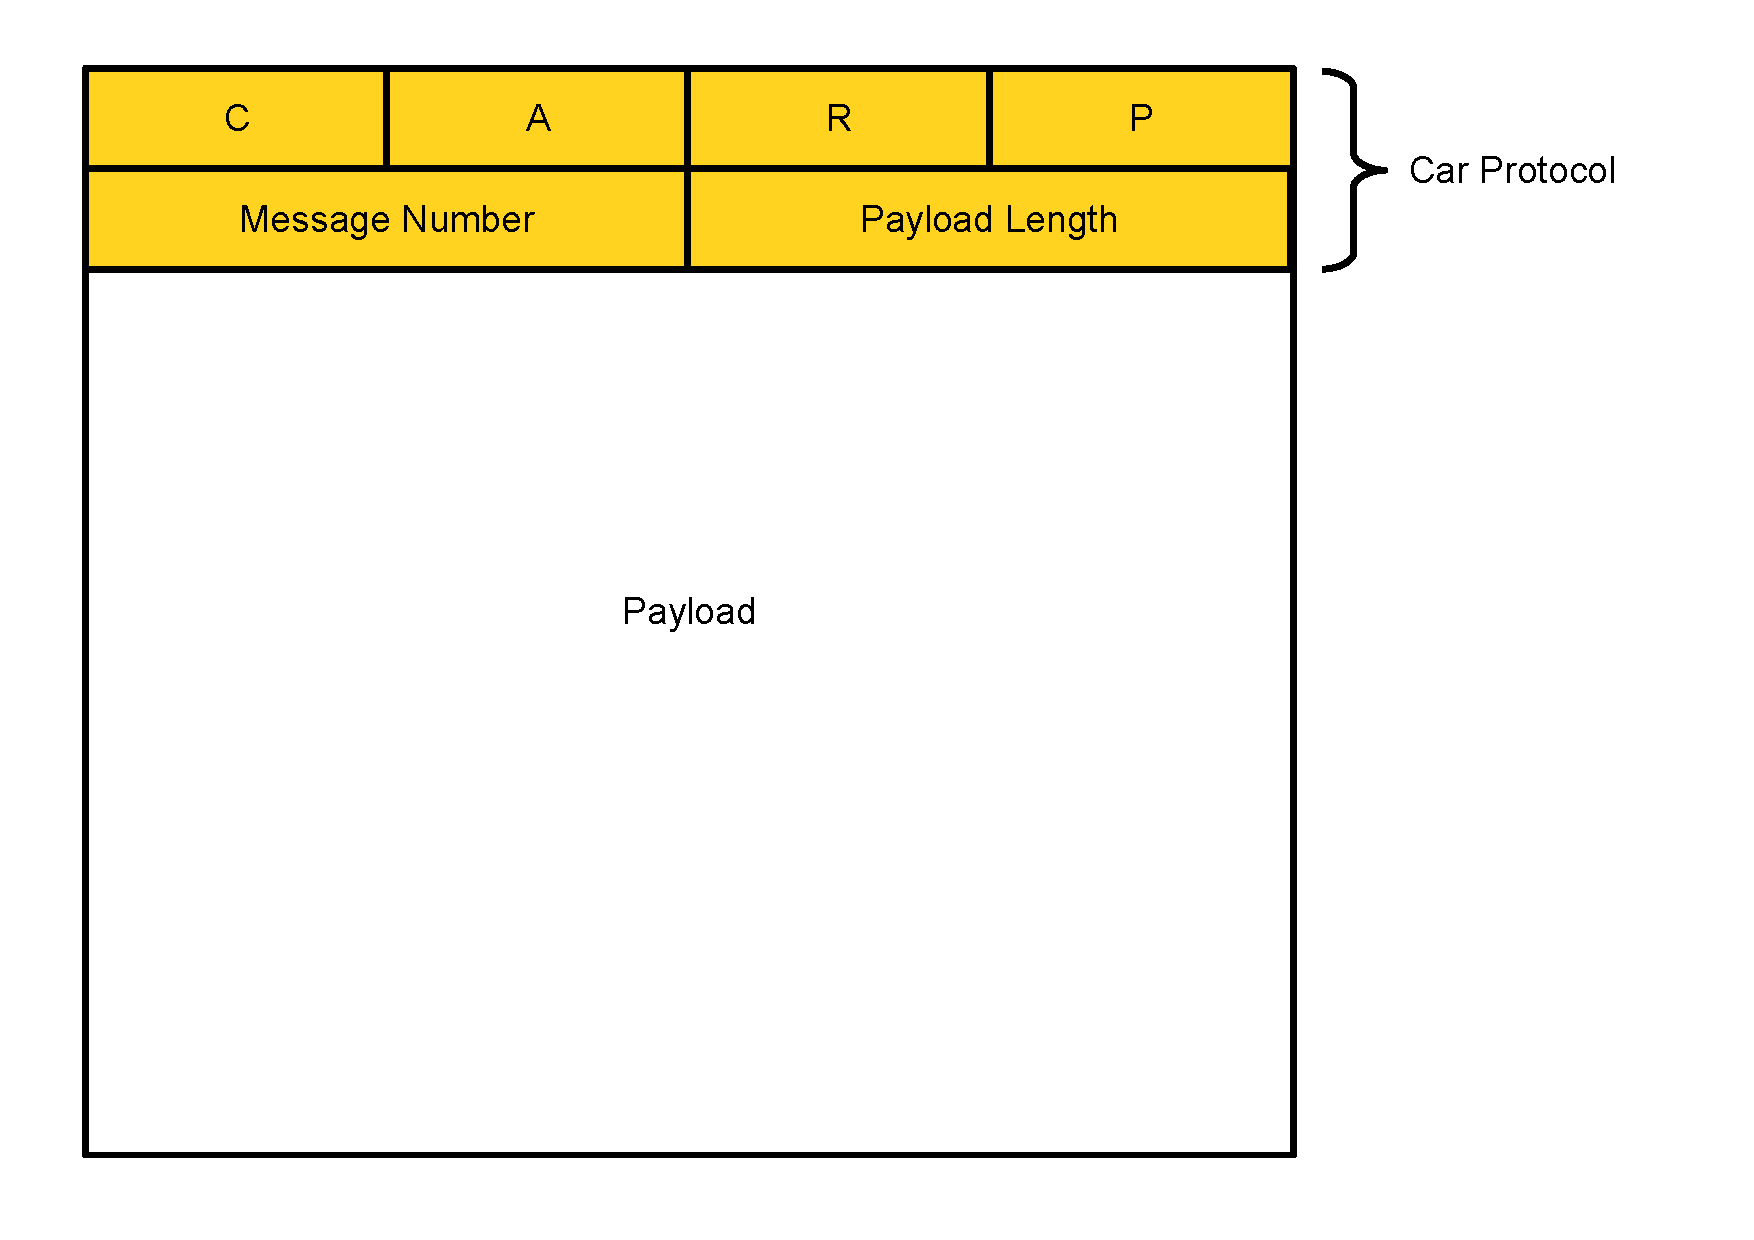
\includegraphics[width=0.5\textwidth]{figures/prot0.pdf}
	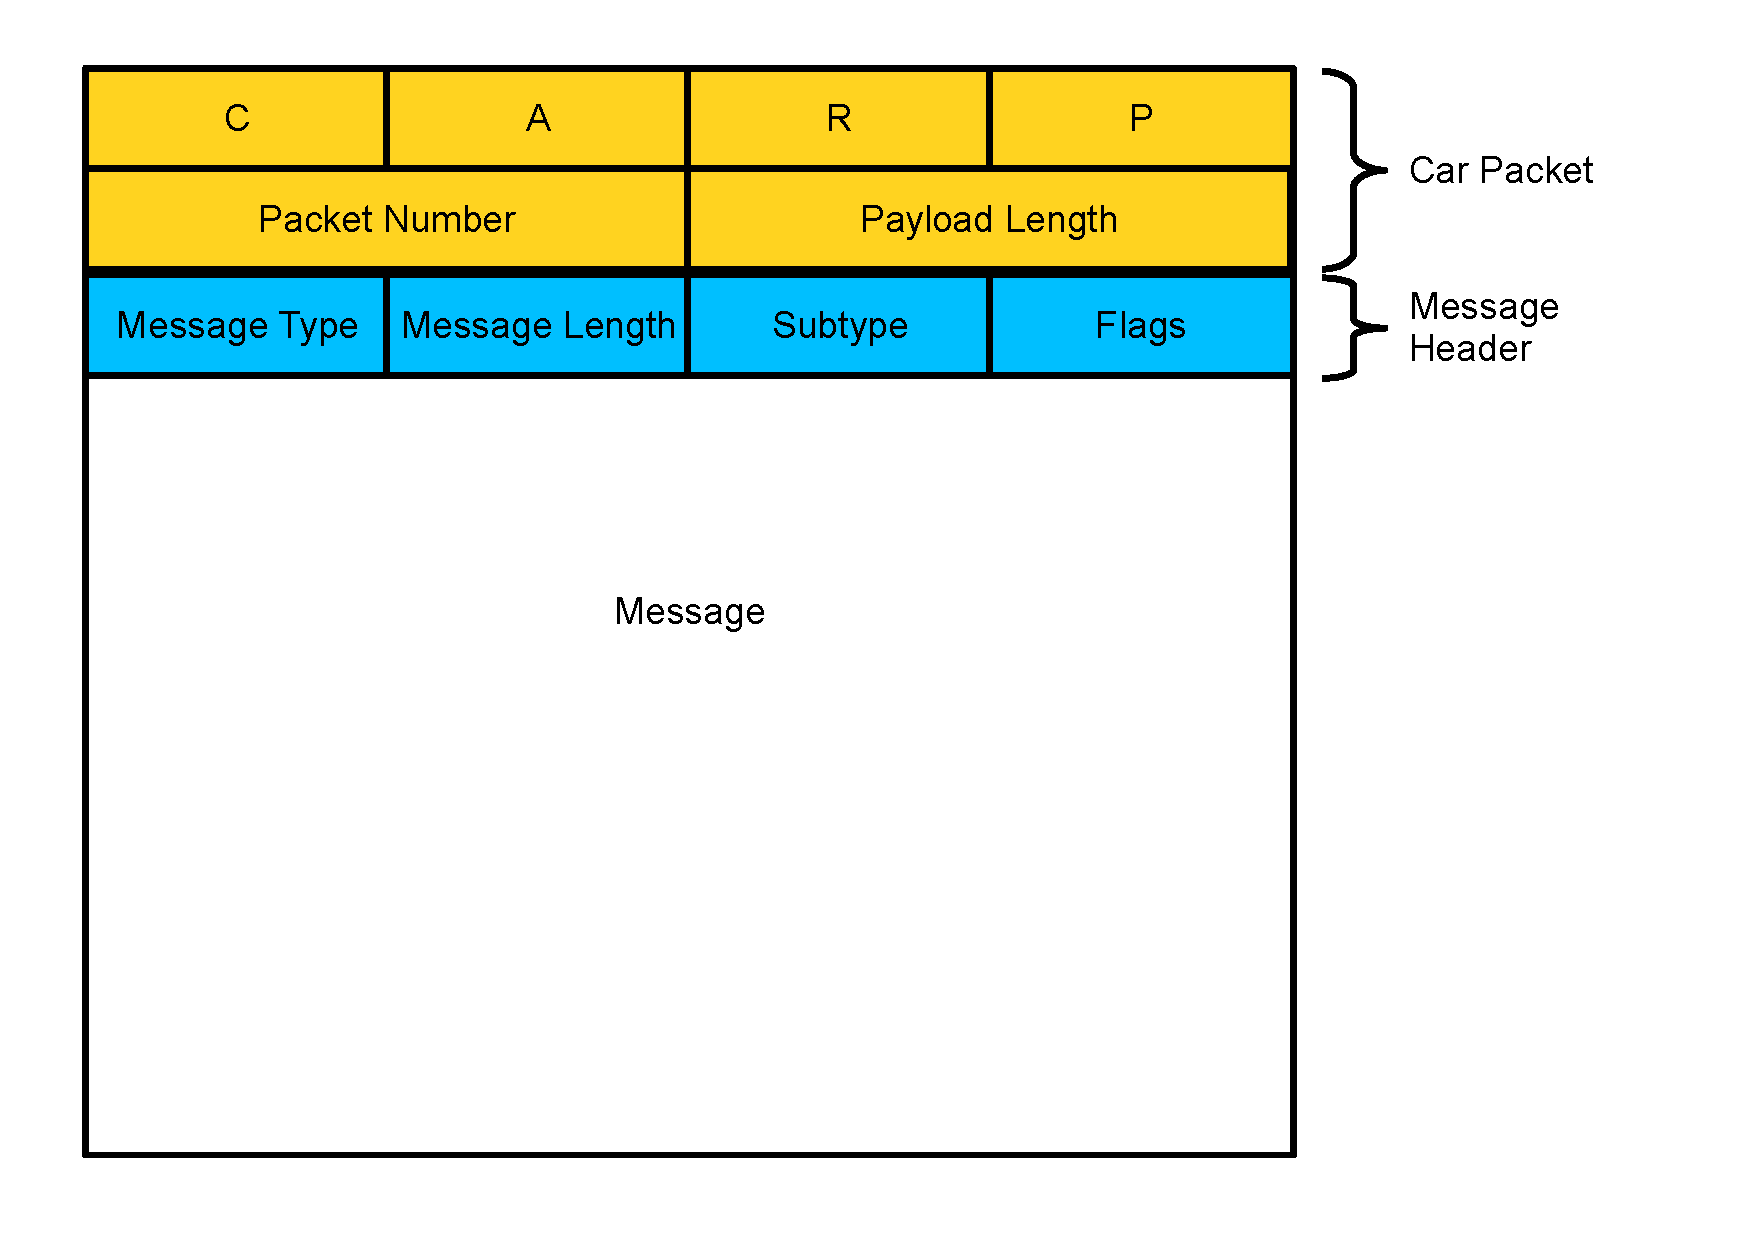
\includegraphics[width=0.5\textwidth]{figures/prot1.pdf}
	\caption{Left: CarProtocol header. Right: CarMessage header.} \label{CarProtocol}
\end{figure}

Packet fields:
\begin{itemize}
\item 'C' 'A' 'R' 'P':\\
Start sequence of the packet to detect a packet in the  incoming byte-stream.
\item PacketNumber:\\
Consecutive increasing 16 bit number which works as an ID. The number is never changed by the Nios2, only by the central ECU (Linux-PC). Thereby the central ECU can detect a protocol fail if the response packet has not the same PacketNumber as the request packet.\\
Please remember the wrap around after the PacketNumber 65535!
\item PayloadLength:\\
Total length of the payload in Bytes. This length information contains not the packet-header length!
\end{itemize}

The payload contains at least one message and max. 8 messages. All messages start at a multiple of 4 assuming that all messages have a multiple of 4 as length. There must be no gap between two messages!!\\

The order of the messages in a packet is important:\\
Contains the packet a WelcomeMessage this message as to be the first. All other messages in this packet will be ignored! Otherwise the first message is the most important followed by the second and so on... The meaning of 'important' was already described in section 4.2.3.\\

Note: As the velocity-message is the most important in normal mode it will be assumed to be the first message!

\subsubsection{CarMessage - Requests and answers}

A CarMessage is the atomic communication part. The central ECU writes some (request) messages and packs them into a CarProtocol packet. The packet is transferred and read by the Nios2 processor. Every message is handled in one of the small cycle runs. Handled means that the message activates a sensor. This sensor fills the empty fields of the message. We called this filled message answer although it looks exactly like the request.\\

Every sensor understands at least one message type. So we send only those messages to a specific FPGA which can be understand by a connected sensor. For example: Only one FPGA has an A/D-Converter so only this FPGA gets a packet with an ADCMessage.\\

A message consists of a message-header and a message-body. The message-header is implemented in a super-class. Due to different body-types the body must be implemented in different subclasses.

The Structure of the message header is shown in \ref{CarProtocol} and described in the following:

\begin{itemize}
\item Type is the ID of the message class. The type follows this rule:
	\begin{itemize}
		\item Types between 0 and 3 are for NETWORKING (such as WelcomeMessage)
		\item Types between 4 and 7 are BASIC messages and have to be understood by every networking client
		\item Types between 8 and 255 are GENERAL purpose messages
	\end{itemize}

\item Length = Length of header (always 4 bytes) + Length of PAYLOAD\\
The Length of request and answer should always be identical!

\item SubType:\\
If a sensor requires more than one message type, SubType distinguishes between this messages. Is there just one message type this field should be 0.

\item Flags: Bits are numbered from 0 (least significant bit) to 7:\\
Bit 0:  Request(0) / Answer(1)
\end{itemize}

\subsubsection{WelcomeMessage}

One example of a CarMessage is the WelcomeMessage. This message has two aims:
\begin{enumerate}
\item Synchronize the 4 Motor-ECU with the central-ECU and
\item inform the central-ECU about the messages which can be understood by this Motor-ECU.
\end{enumerate}

The central-ECU sends (at the same time) a WelcomeMessage to each Motor-ECU. The Motor-ECUs
answer with the same message but additional with a list of those messages which are available
at this ECU. The list is marked with Operation 1, Operation 2, ...\\

The message has the structure given in \ref{WelcomeMessage}.

\begin{figure}[ht]
	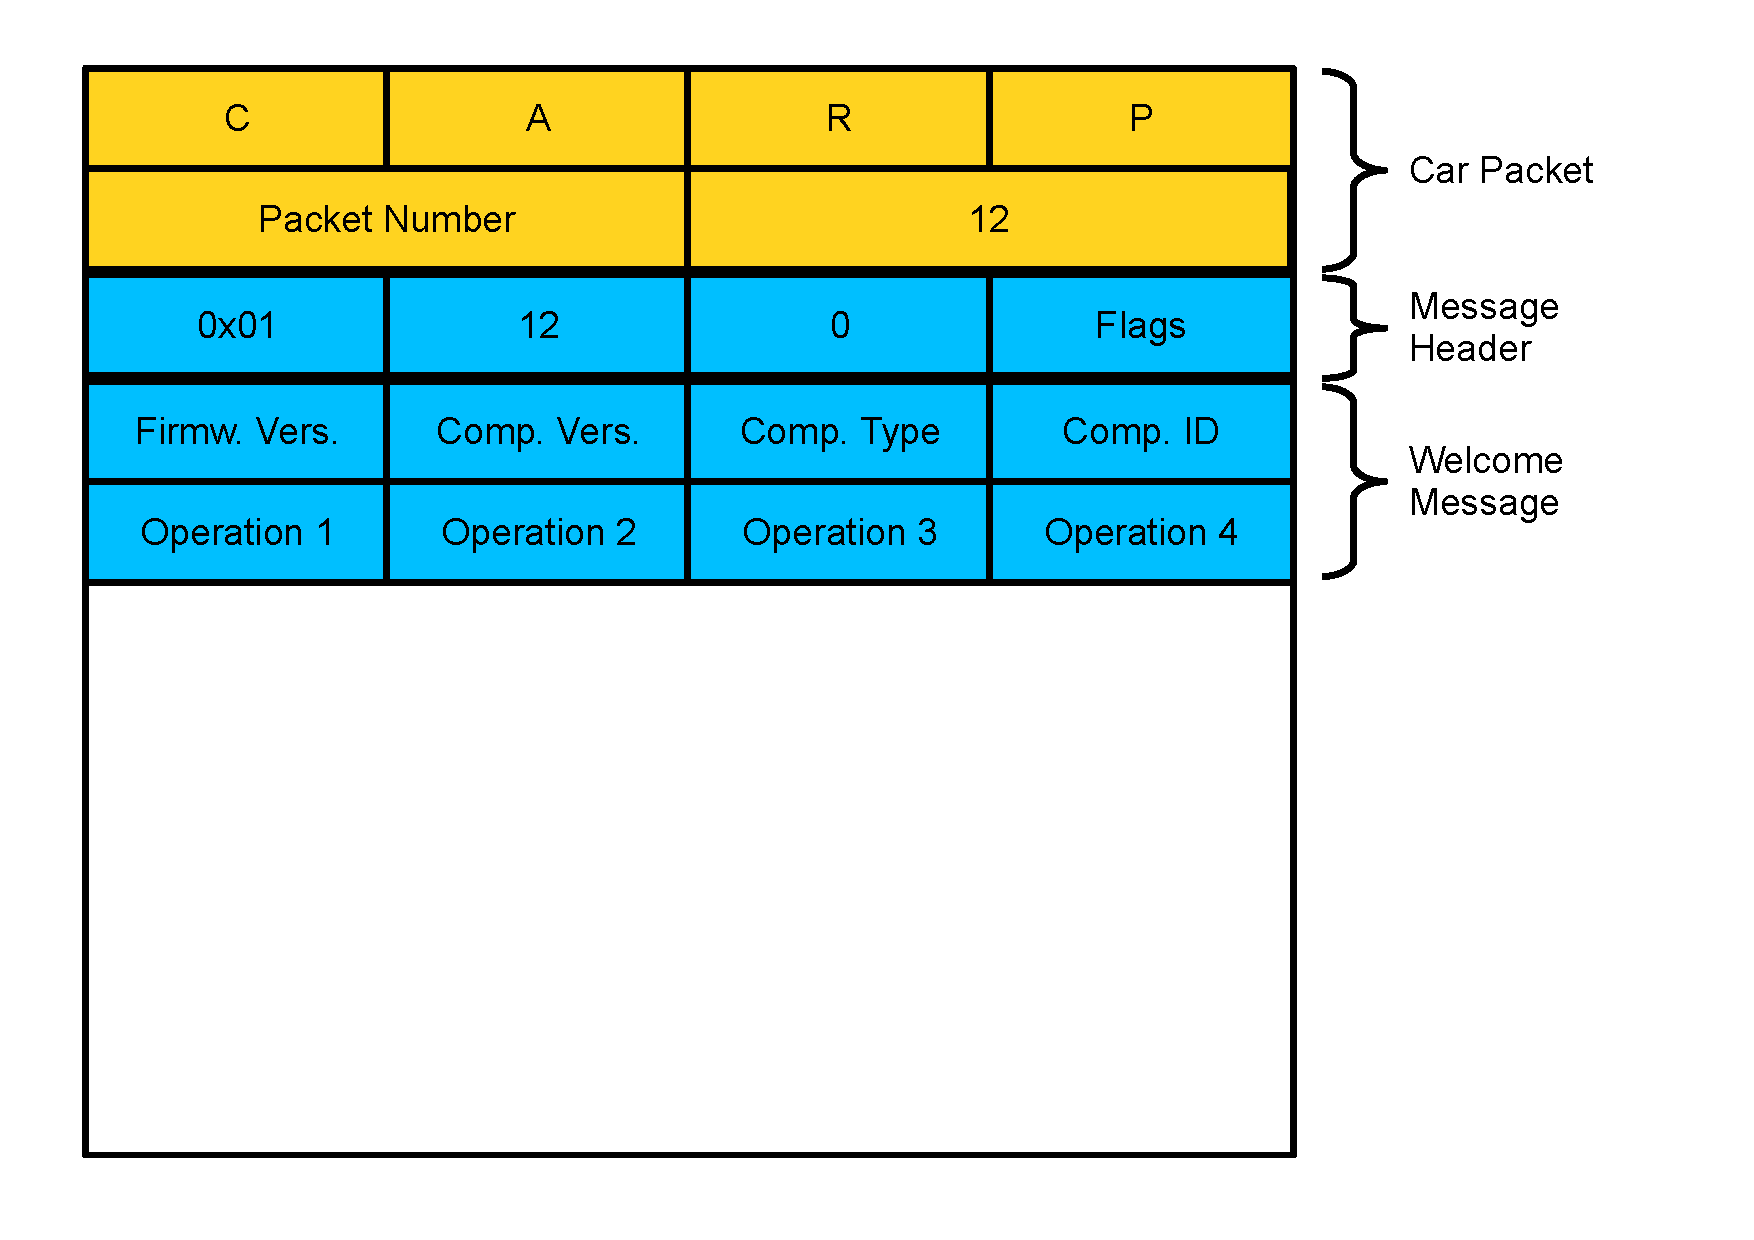
\includegraphics[width=0.5\textwidth]{figures/prot2.pdf}
	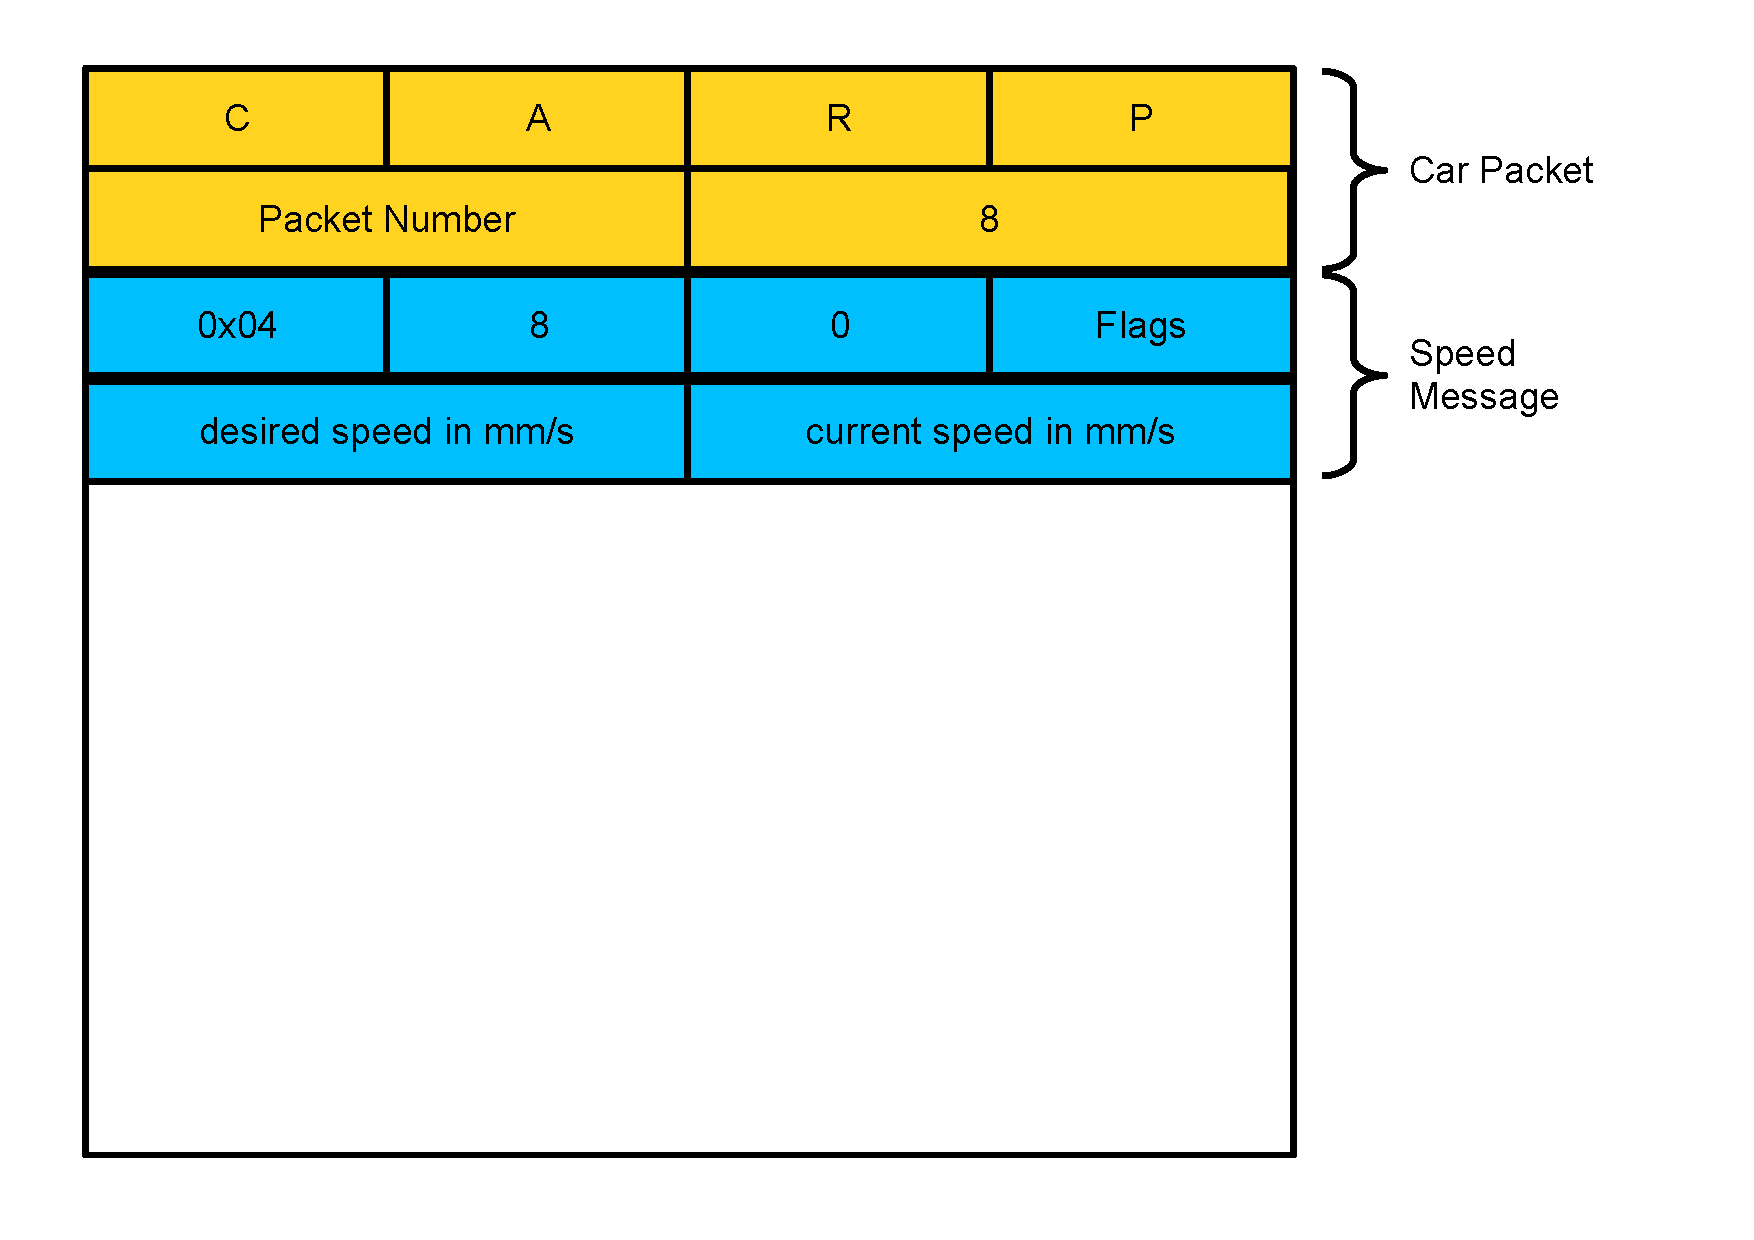
\includegraphics[width=0.5\textwidth]{figures/prot3.pdf}
	\caption{Left: WelcomeMessage. Right: CarVelocityMessage.} \label{WelcomeMessage}
\end{figure}

Only those MessageTypes are necessary to list in the WelcomeMessage with a type $>=$ 8.
The list has to be filled up with 0x00 if less then 4 additional messages are understood.

\begin{figure}[ht] 
	\center{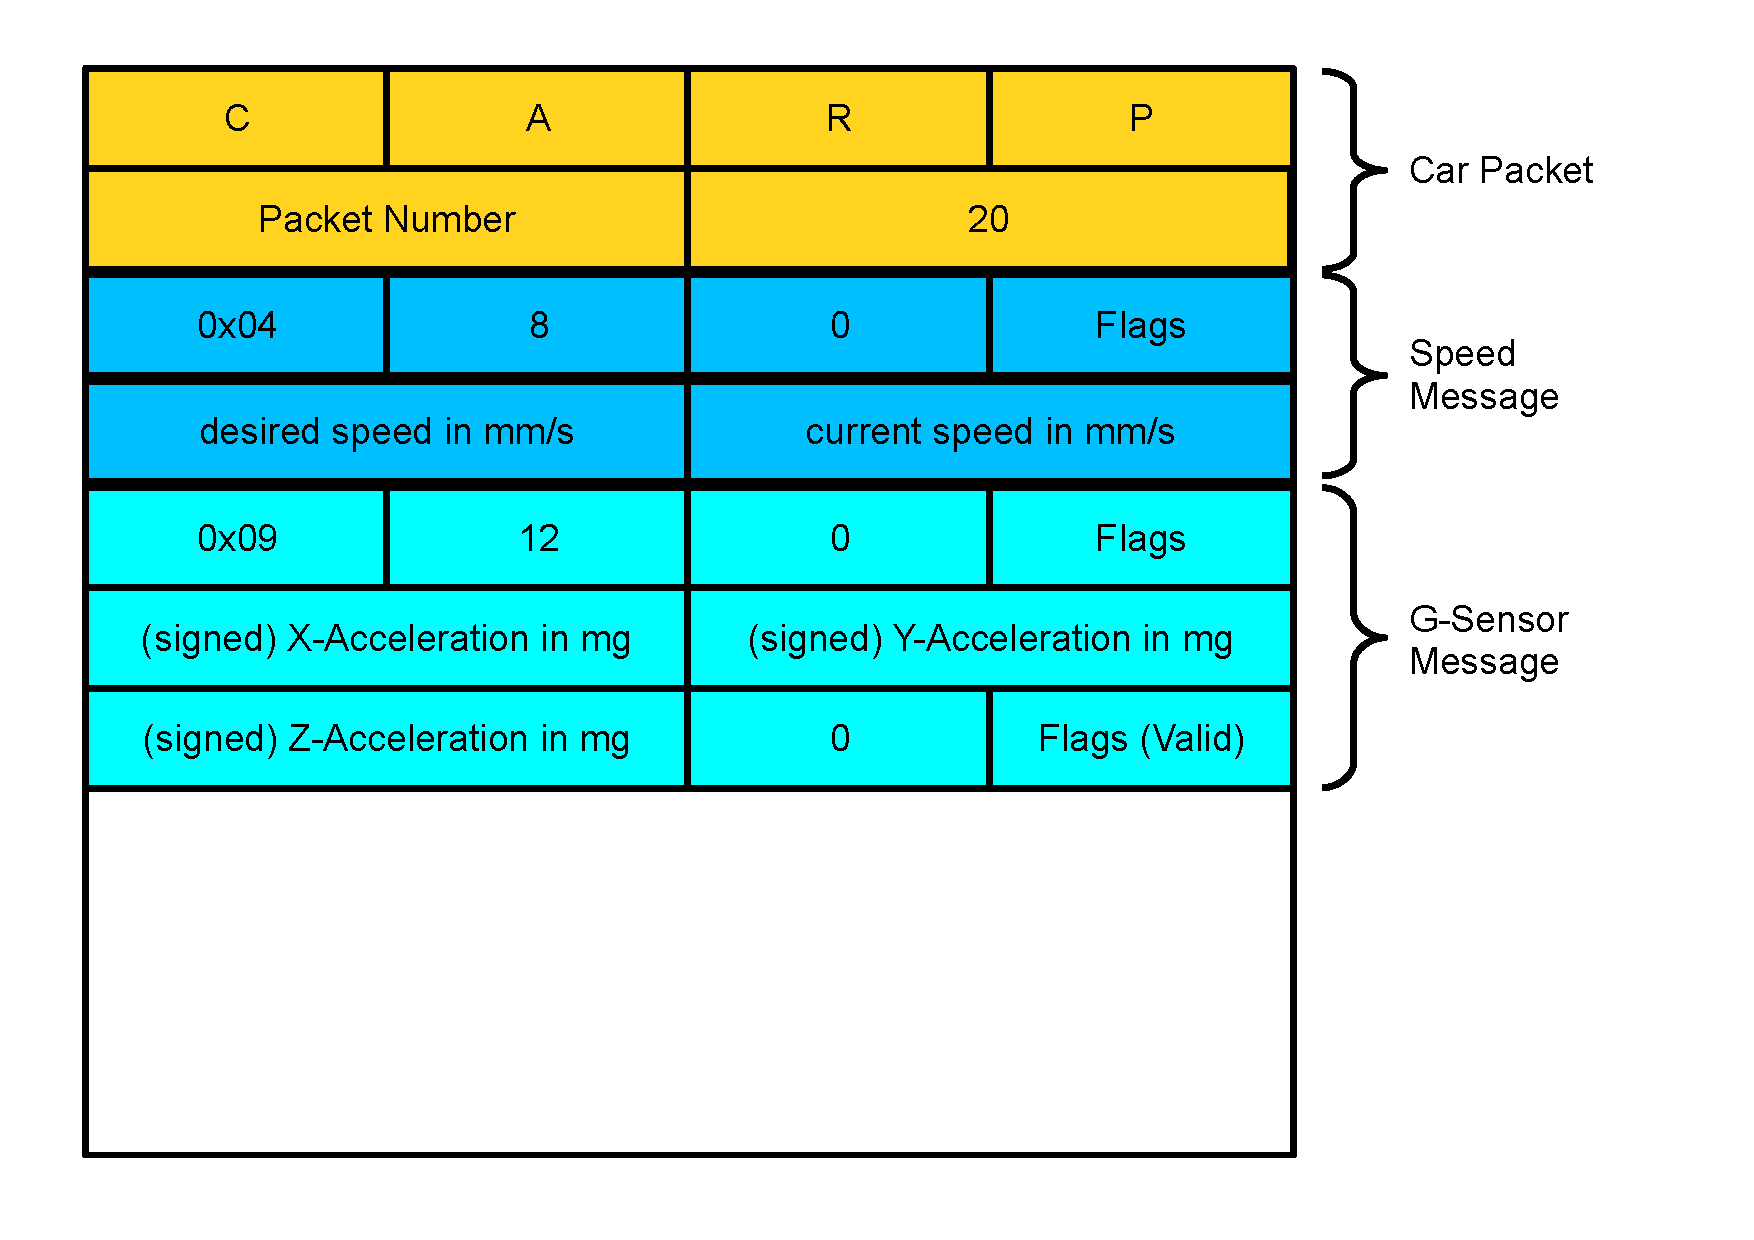
\includegraphics[width=0.5\textwidth]{figures/prot4.pdf}}
	\caption{Two messages in one packet.} \label{example}
\end{figure}

\subsubsection{Another example: CarVelocityMessage}

For another example see \ref{WelcomeMessage} right and \ref{example}.

\subsection{Central ECU: Networking interface}

\subsubsection{Overview}

We decided to separate path-planning and communication. Therefore we developed the system structure given in \ref{linuxPC}.

\begin{figure}[p]
	\center{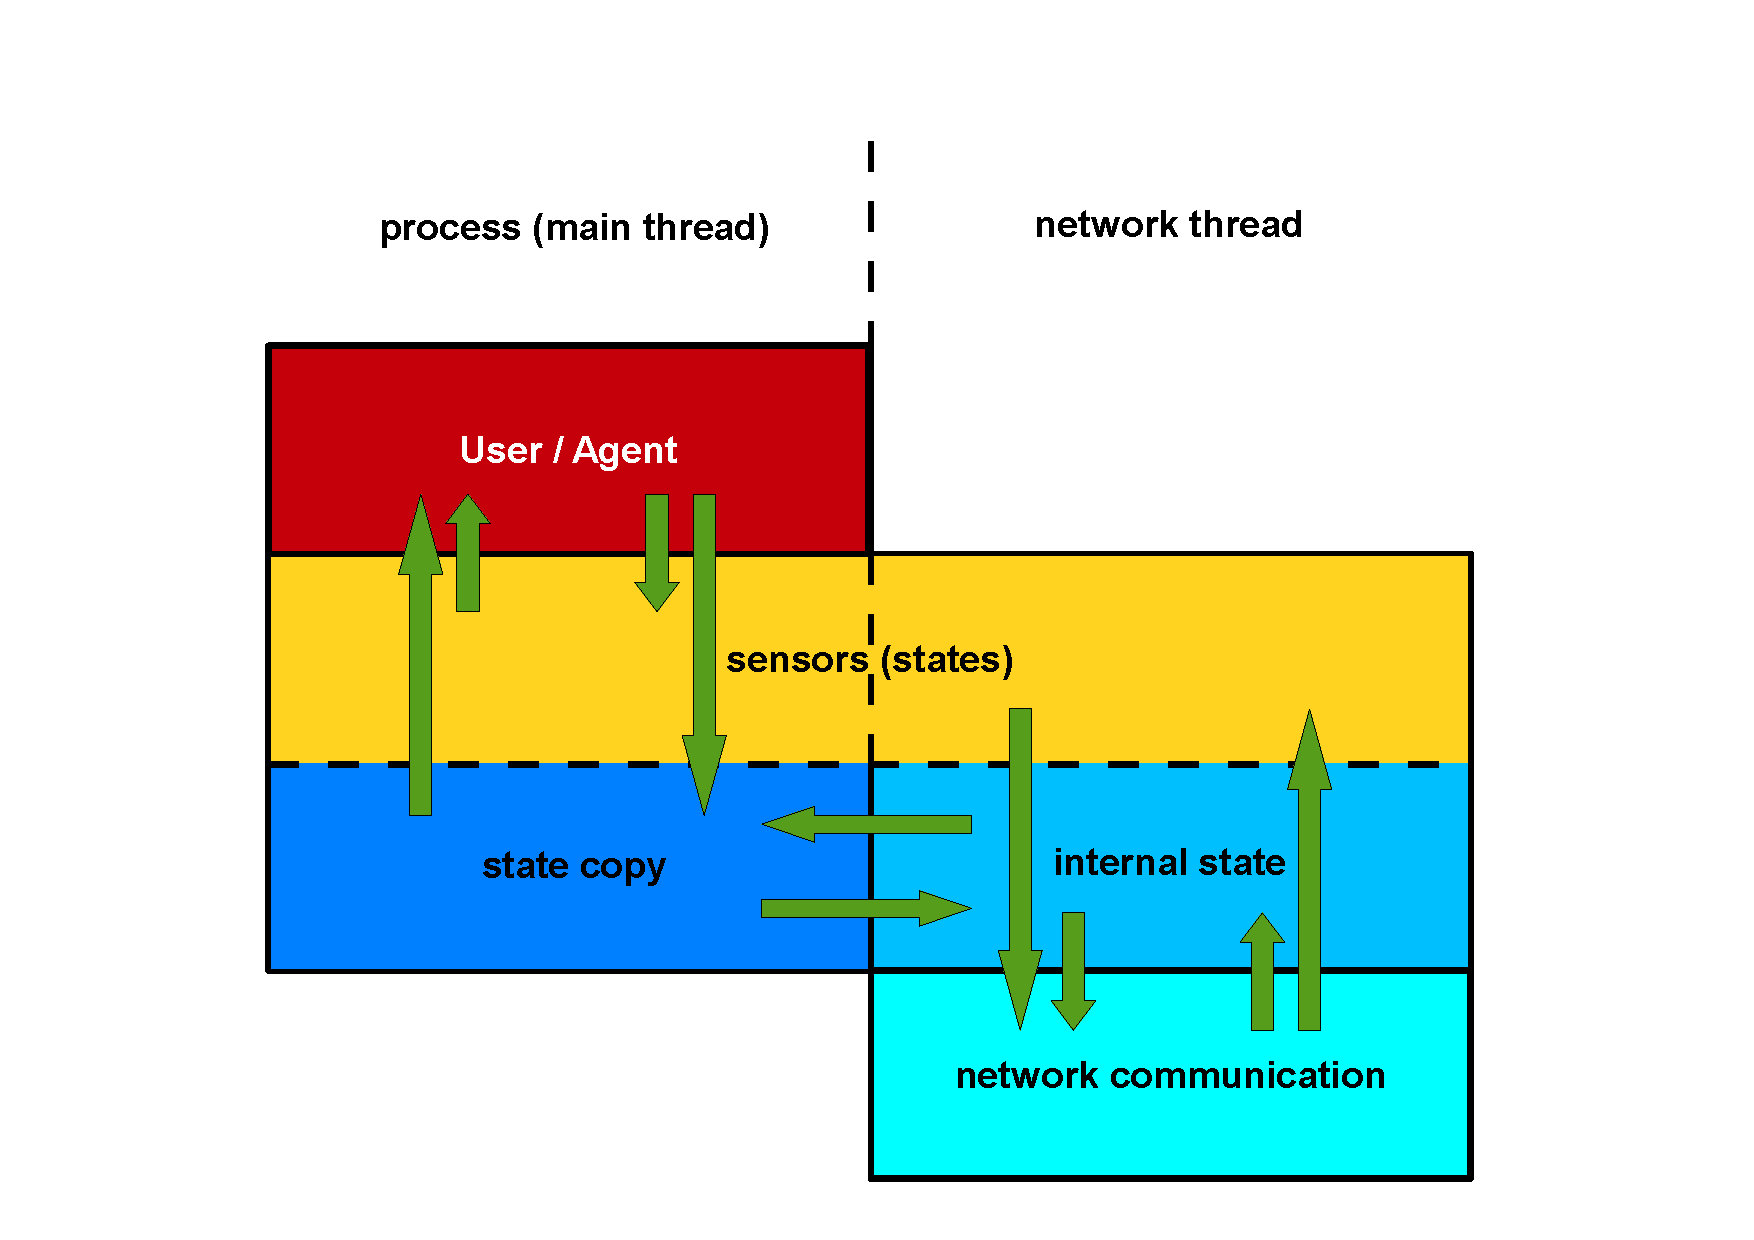
\includegraphics[width=\textwidth]{figures/linuxPC_structure.pdf}}
	\caption{The software structure on the Linux-PC.} \label{linuxPC}
\end{figure}

We are using two threads in the process. The first one is the main thread driving the user- or agent-program. The second one drives the networking. The aim is that the user can use a struct or class which represents the current state of the car.\\

The said state consists of:
\begin{itemize}
	\item General information, such as version, connected sensors, ...
	\item Motor information, such as current speed, max. speed, PID-values
	\item current state of the connected sensors
\end{itemize}

The current state of the connected sensors is represented in an own class (see below).\\

\subsubsection{Network Thread}

This thread initializes the communication (see WelcomeMessage) and polls information from the car. With the received answers it updates an thread-internal state. But how does this thread generate the necessary messages?\\

The answer of the WelcomeMessage contains a list of the available sensor types (message types). The network thread generates a sensor representation of each sensor type. This representation derives from the super-class called SensorState. So we know the sensor types. How about the messages?\\

SensorState has two important methods: 
\begin{itemize}
	\item[] virtual CCarMessage *getCarMessage()
	\item[] virtual bool updateSensorState(CCarMessage * p\_message)
\end{itemize}

These methods are used to generate the necessary messages and to update the sensor state with the received answer.\\

So the main task of the networking thread is collecting the messages from the SensorState objects, packing them into a packet and sending it to the motor-ECUs. After receiving a packet, it is spitted back and every sensor is updated with the answer. See \ref{sensors} for the complete communication chain.

\begin{figure}[p]
	\center{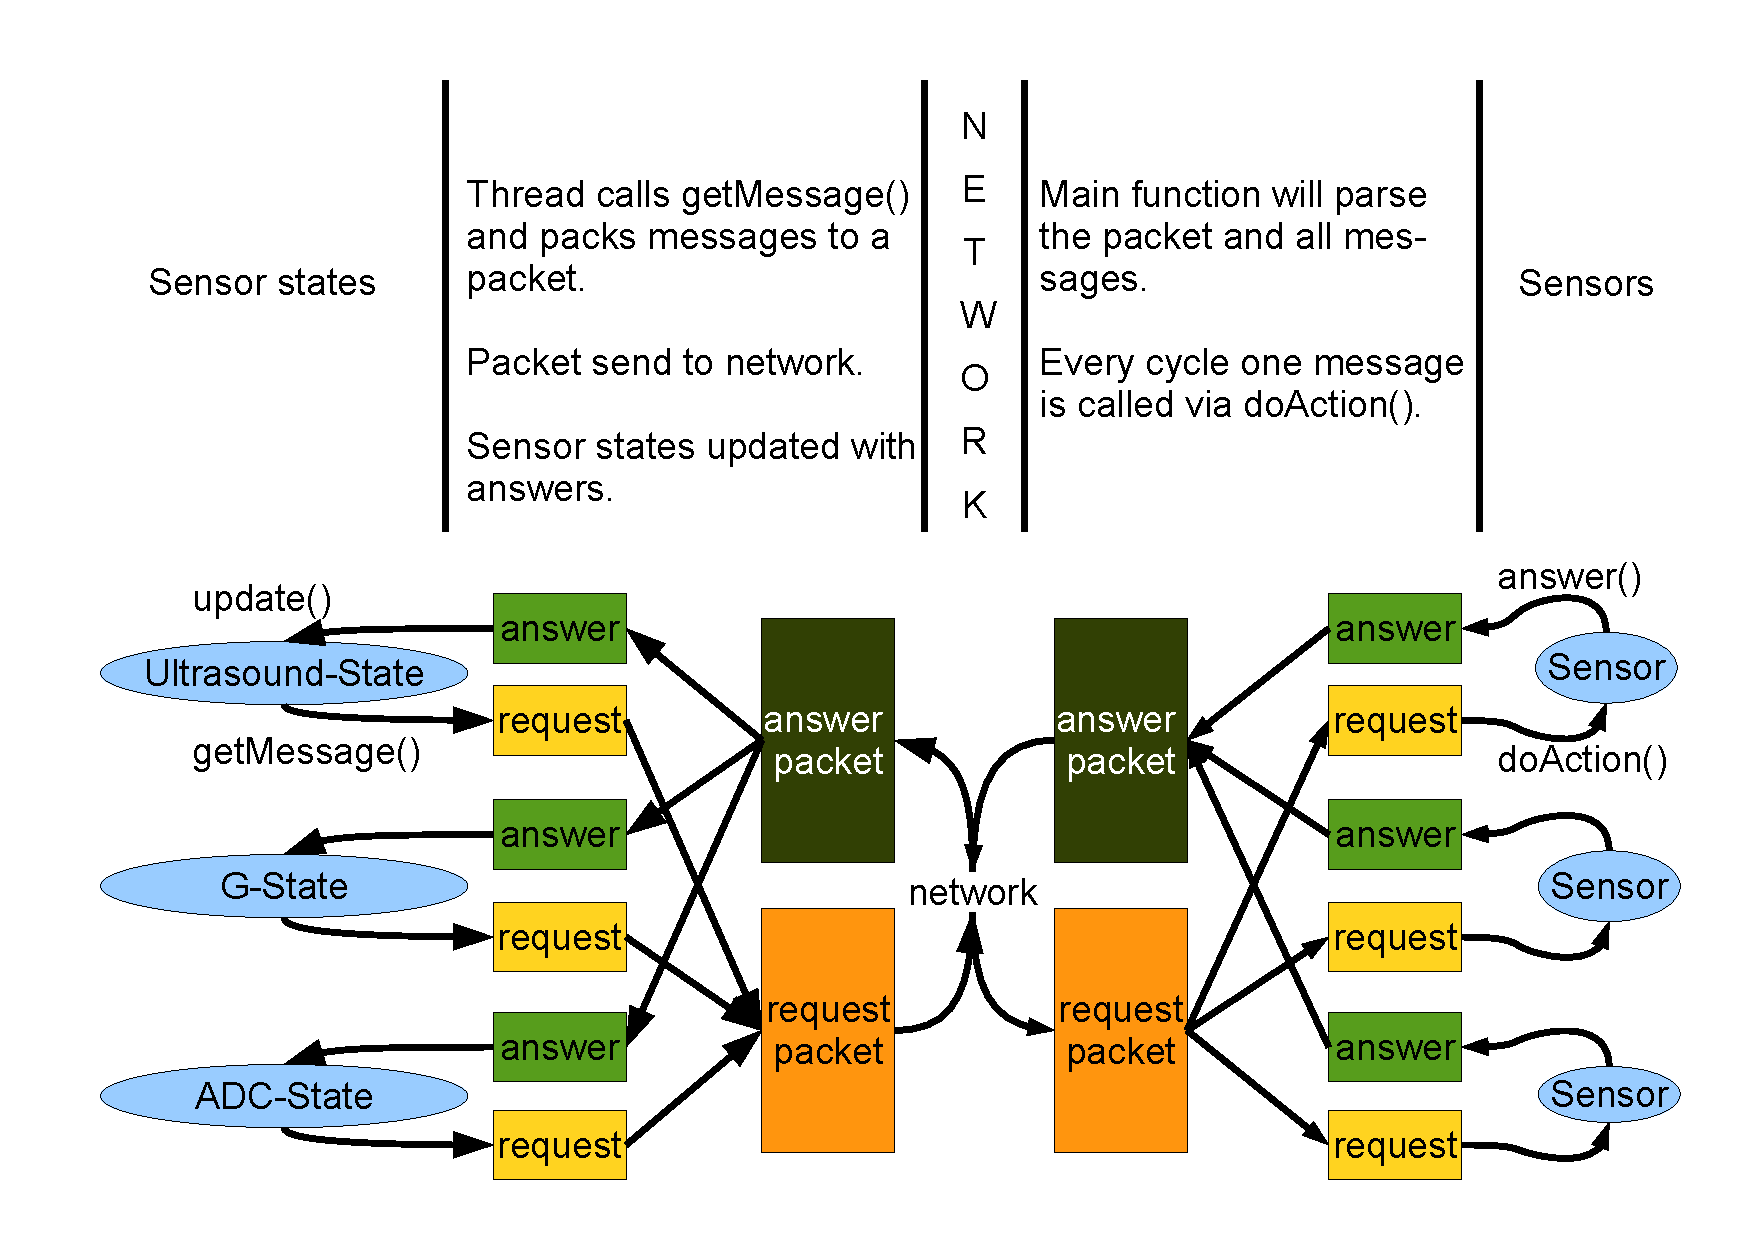
\includegraphics[width=\textwidth]{figures/messageChain.pdf}}
	\caption{The sensor structure and message chain in the whole project.} \label{sensors}
\end{figure}

\subsubsection{Main Thread}

The main thread can get a copy from the said internal state. The used function is (of course) thread safe. The copy will be done with memcpy(..).\\

Please Note: The pointers to the sensor states are always the same as in the internal state. So the sensor states are updated automatically, but the static information (current speed, ...) not. The sensor states must be thread safe as well!\\
Maybe someone can introduce copy-constructors on the sensor states to solve this issue.\\

So the proper way of controlling the car is the following:
\begin{enumerate}
 \item Call startConnection() // Enables networking and starts new Thread
 \item Allocate space for one Car\_State object
 \item Call getState(..) with the said object. You will get a copy of the current state
 \item Call the sensors (Car\_State.motorStates[i].p\_sensors[j]->get....()) for additional state information (distance, ADC values, ...)
 \item Use the information to do something.
 \item Get a more actual copy of the internal state by calling getState() once again.
 \item Set something in this copy to a new value (e.g. set a new desired\_speed).
 \item Call setState(..) to transfer your changes.\\
 It takes some time that the car adopts the new values (see message delay).
 \item Return to step 3. or call stopConnection() before program exit.\\
\end{enumerate}


\subsection{Central ECU: User-/Agent-View}

Processing Unit: \textsl{Sabre-light i.mx6} development board (4 cores).\\
	
Main tasks:
\begin{enumerate}
	\item Control the speed-controller
	\item (Polling the sensors)
	\item Calculate next behavior
\end{enumerate}

\subsubsection{Software Architecture}

\begin{itemize}
	\item Multi-Process / Multi-Thread
	\item seperated Behavior-Planning and Network-Communication
\end{itemize}

\subsubsection{Current setup}

\begin{itemize}
	\item Main application: 
	\begin{itemize}
		\item 1. Thread: network-communication
		\item Main Thread: behavior-planning (exploration mode)
	\end{itemize}		 
	\item dhcp-server, os, much more ;)
\end{itemize}

\subsubsection{Current behavior}

\begin{itemize}
	\item The car should be driving in one direction. 
	\item Is there an obstacle it turns left until the obstacle is not in it's way anymore. 
	\item Then the car drives further in this direction.
	\item If car is in danger (see wall) then the car will speed down.
	\item If the distance between car and obstacle is lower 20 cm then the car will stop.
\end{itemize}

\subsubsection{Possible behavior}

Remote control mode:
\begin{itemize}
	\item Human user controls movements via GUI
	\item GUI sends data to a hidden server (not NSA)
	\item If car is in danger (see wall ;)) then the car will speed down.
	\item If the distance between car and obstacle is lower 20 cm then the car will stop.
\end{itemize}

Other possible behavior:
\begin{itemize}
	\item ABS, ESP via G-Sensors (data is already available)
	\item Web-Cam for little NSA-agents ;)
	\item ...
\end{itemize}


